\section{Related Work}\label{sec:related_work}

\subsection{Commit Reveal Scheme}\label{sec:related_work_commit_reveal}

The commit reveal scheme is a decentralized protocol for generating verifiable random numbers. Let $\varepsilon$ denote entropy and $P$ represent a provider. The Provider Set is defined as:
\begin{equation}
\mathcal{P} = \{p_1, p_2, ..., p_n\}
\end{equation}

A commitment is defined as the hash of an entropy value:
\begin{equation}
c_i = \text{hash}(\varepsilon_i)
\end{equation}
where $c_i$ is the commitment from provider $p_i$. The protocol is executed through a secure smart contract that handles the aggregation of provider entropy values.

\begin{figure}[h]
\centering
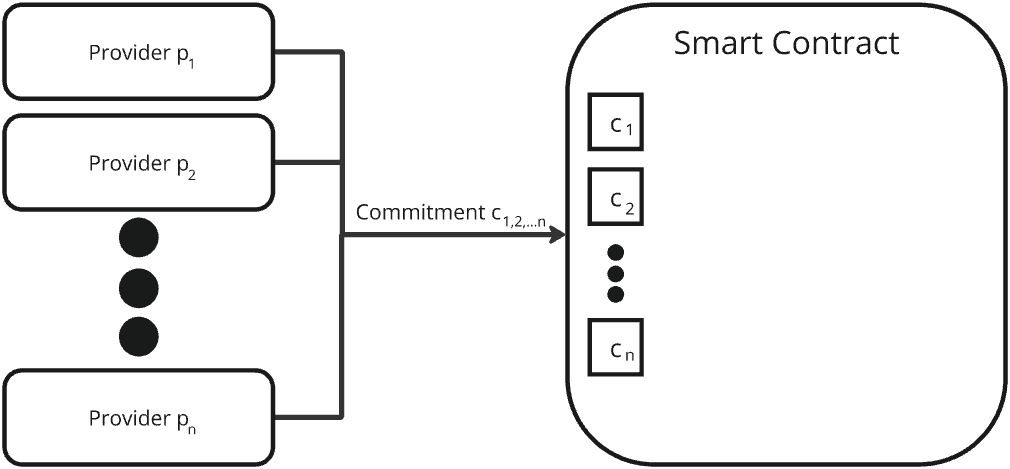
\includegraphics[width=0.8\textwidth]{images/commitment-stage.png}
\caption{Commitment Stage: Providers simultaneously submit hash commitments of their entropy values}
\label{fig:commitment-stage}
\end{figure}

\begin{figure}[h]
\centering
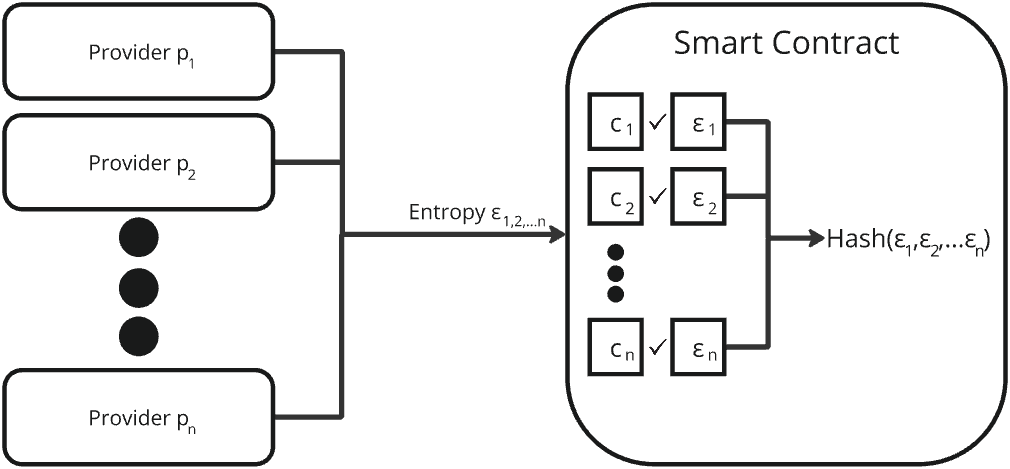
\includegraphics[width=0.8\textwidth]{images/reveal-stage.png}
\caption{Reveal Stage: Providers reveal their original entropy values which are verified against their commitments. After verification, a verifiable entropy unknown to any individual provider is created using a hash function}
\label{fig:reveal-stage}
\end{figure}

The protocol consists of the following key steps:

\begin{enumerate}
    \item \textbf{Provider Commitment}: Each provider $p_i$ commits to their entropy by submitting $c_i = \text{hash}(\varepsilon_i)$ to the smart contract
    \item \textbf{Provider Entropy}: After all commitments are received, providers reveal their original entropy values $\varepsilon_i$
    \item \textbf{Verification}: The smart contract verifies each revealed entropy matches its commitment by checking $c_i = \text{hash}(\varepsilon_i)$
    \item \textbf{Entropy Aggregation}: After all submitted entropies are verified, a verifiable entropy unknown to any of the individual providers is created using a method such as a hash function
\end{enumerate}

\subsubsection{Naive Implementation Vulnerability}\label{sec:commit_reveal_vulnerability}

While this naive commit-reveal scheme achieves decentralization, it suffers from a critical any-malicious denial of service vulnerability. Consider the following lottery scenario:

Suppose a lottery is being conducted with an insurmountable monetary reward. A single malicious provider can exploit the protocol through the following attack vector:

\begin{enumerate}
    \item The malicious provider initially follows the protocol through the commitment step, submitting their hash commitment like other participants.

    \item During the entropy revelation step, this provider (who may have purchased any number of lottery tickets) can wait until all other providers have revealed their entropy values.

    \item At this moment, the malicious actor can calculate the final outcome of the lottery by combining:
    \begin{itemize}
        \item All revealed entropy values from honest providers
        \item Their own private (yet unrevealed) entropy
    \end{itemize}

    \item With knowledge of the final outcome, the malicious actor can:
    \begin{itemize}
        \item If favorable: reveal their entropy and allow the lottery to complete
        \item If unfavorable: withhold their entropy, forcing a protocol restart and a new chance at a favorable outcome
    \end{itemize}
\end{enumerate}

This vulnerability demonstrates how a single malicious actor can repeatedly force redraws until achieving their desired outcome, effectively compromising the fairness of any high-stakes random number generation. Replacing the hash commitment with a time-lock puzzle closes it: the withheld value can always be recovered, so withholding no longer changes the outcome.

\subsection{Oracle Based VRF}\label{sec:oracle_based_vrf}
Chainlink's Verifiable Random Function (VRF)~\cite{chainlink_vrf} is based on the VRF construction proposed by Goldberg et al.~\cite{goldbergVRF}. The Goldberg VRF creates a pseudorandom number that is verifiable by the public. However, as noted in their work, it ``guarantees that $\beta$ is indistinguishable from random by anyone who does not know the secret key SK.'' Conversely, this implies that anyone in possession of the secret key can predict the ''random'' output.

This reliance on secret key holder(s) creates a fundamental trust assumption. Chainlink's implementation depends entirely on the trustworthiness of Chainlink and their ability to secure their secret key from hackers and corruption, creating a single point of failure.

\subsection{Threshold Signature Beacons}\label{sec:threshold_beacons}
A threshold beacon splits one signing key across $n$ parties so that any $t$ of them can sign a round number, and the unique BLS signature of that round becomes its random value. No single party can bias the output and missing parties do not stop it. The trust assumption, however, is $t$-of-$n$: any $t$ colluding parties can compute every future round in advance. RandAO offers such a beacon as its fast \texttt{quick} tier, for applications where that assumption is acceptable, and keeps the any-honest time-lock beacon for everything else.
